\section{The Large Hadron Collider}
The Large Hadron Collider (LHC) is the proton-proton storage ring operating at CERN and for last 13 years has been the world's highest energy particle collider. The LHC first began operation particles in 2008, but following a magnetic quench incident, it had to be repaired and adjusted, so the first data-taking didn't occur until 2009 \cite{Rossi_2010}. During the 9 years of LHC operation, protons colliding within each of the experiments were increased to larger center-of-mass energies, approaching the design energy of 14TeV. In addition, luminosity has successively been increased, surpassing design luminosity of $1\times10^{34}$cm$^{-2}$s$^{-1}$ in 2018 to reach $2\times10^{34}$cm$^{-2}$s$^{-1}$\cite{CERNnews1}. The overall data recorded in the ATLAS detector totals more than $10^{16}$ collisions. The consistent day-to-day operation of the LHC as well as its strides in increasing the energy and number of collisions produced has led to the most precise measurements of Standard Model constants including the coupling of the Higgs boson to bottom quarks \cite{Aabout_2018_0}, $W$ and $Z$ bosons \cite{Aaboud_2019}, \cite{Aaboud_2018} as well as photons\cite{Aaboud_2018_2} and tau leptons \cite{Aaboud_2019_2}. The LHC has also facilitated searches searches over a wide parameters space, setting confidence level exclusion limits on masses of supersymmetric particles like squarks, gluions and neutralinos \cite{ATLAS-CONF-2019-040}. 

The LHC is set to begin Run 3, in which design center-of-mass energy should be reached, in 2021. Following Run 3, detector upgrades will be made during a long shutdown and then the High-Luminosity LHC (HL-LHC), with unprecedented $10\times$ the luminosity of the LHC, will begin colliding protons in 2027\cite{CERNnews2}. The HL-LHC and its goals will be explained further in \ref{The High-Luminosity LHC and Inner Tracker (ITk)}, suffice to say that LHC-physics is progressing quickly and promises exciting developments in the near future. 

In a brief explanation of the LHC operation, one could begin with the small volume of protons- numbering $\approx 10^{11}$- that is accelerated. Next describe injection, acceleration in PS, SPS, then injection to LHC. 

The LHC basic layout mimics that of the Large Electron Positron collider (LEP) that was housed in the same tunnels prior. Figure \ref{fig:LHClayout} shows the positioning of each experiment on the LHC as well as injection systems and other features. Once proton bunches enter the LHC in two opposing beams they are further accelerated with radio frequency systems. Located at Point 4 in the LHC schematic, the system consists of two cavities operating at twice the frequency of the SPS injector. \textcolor{red}{Brief explanation of RF cavity and how work} 

\begin{figure}[!h]
        \centering
    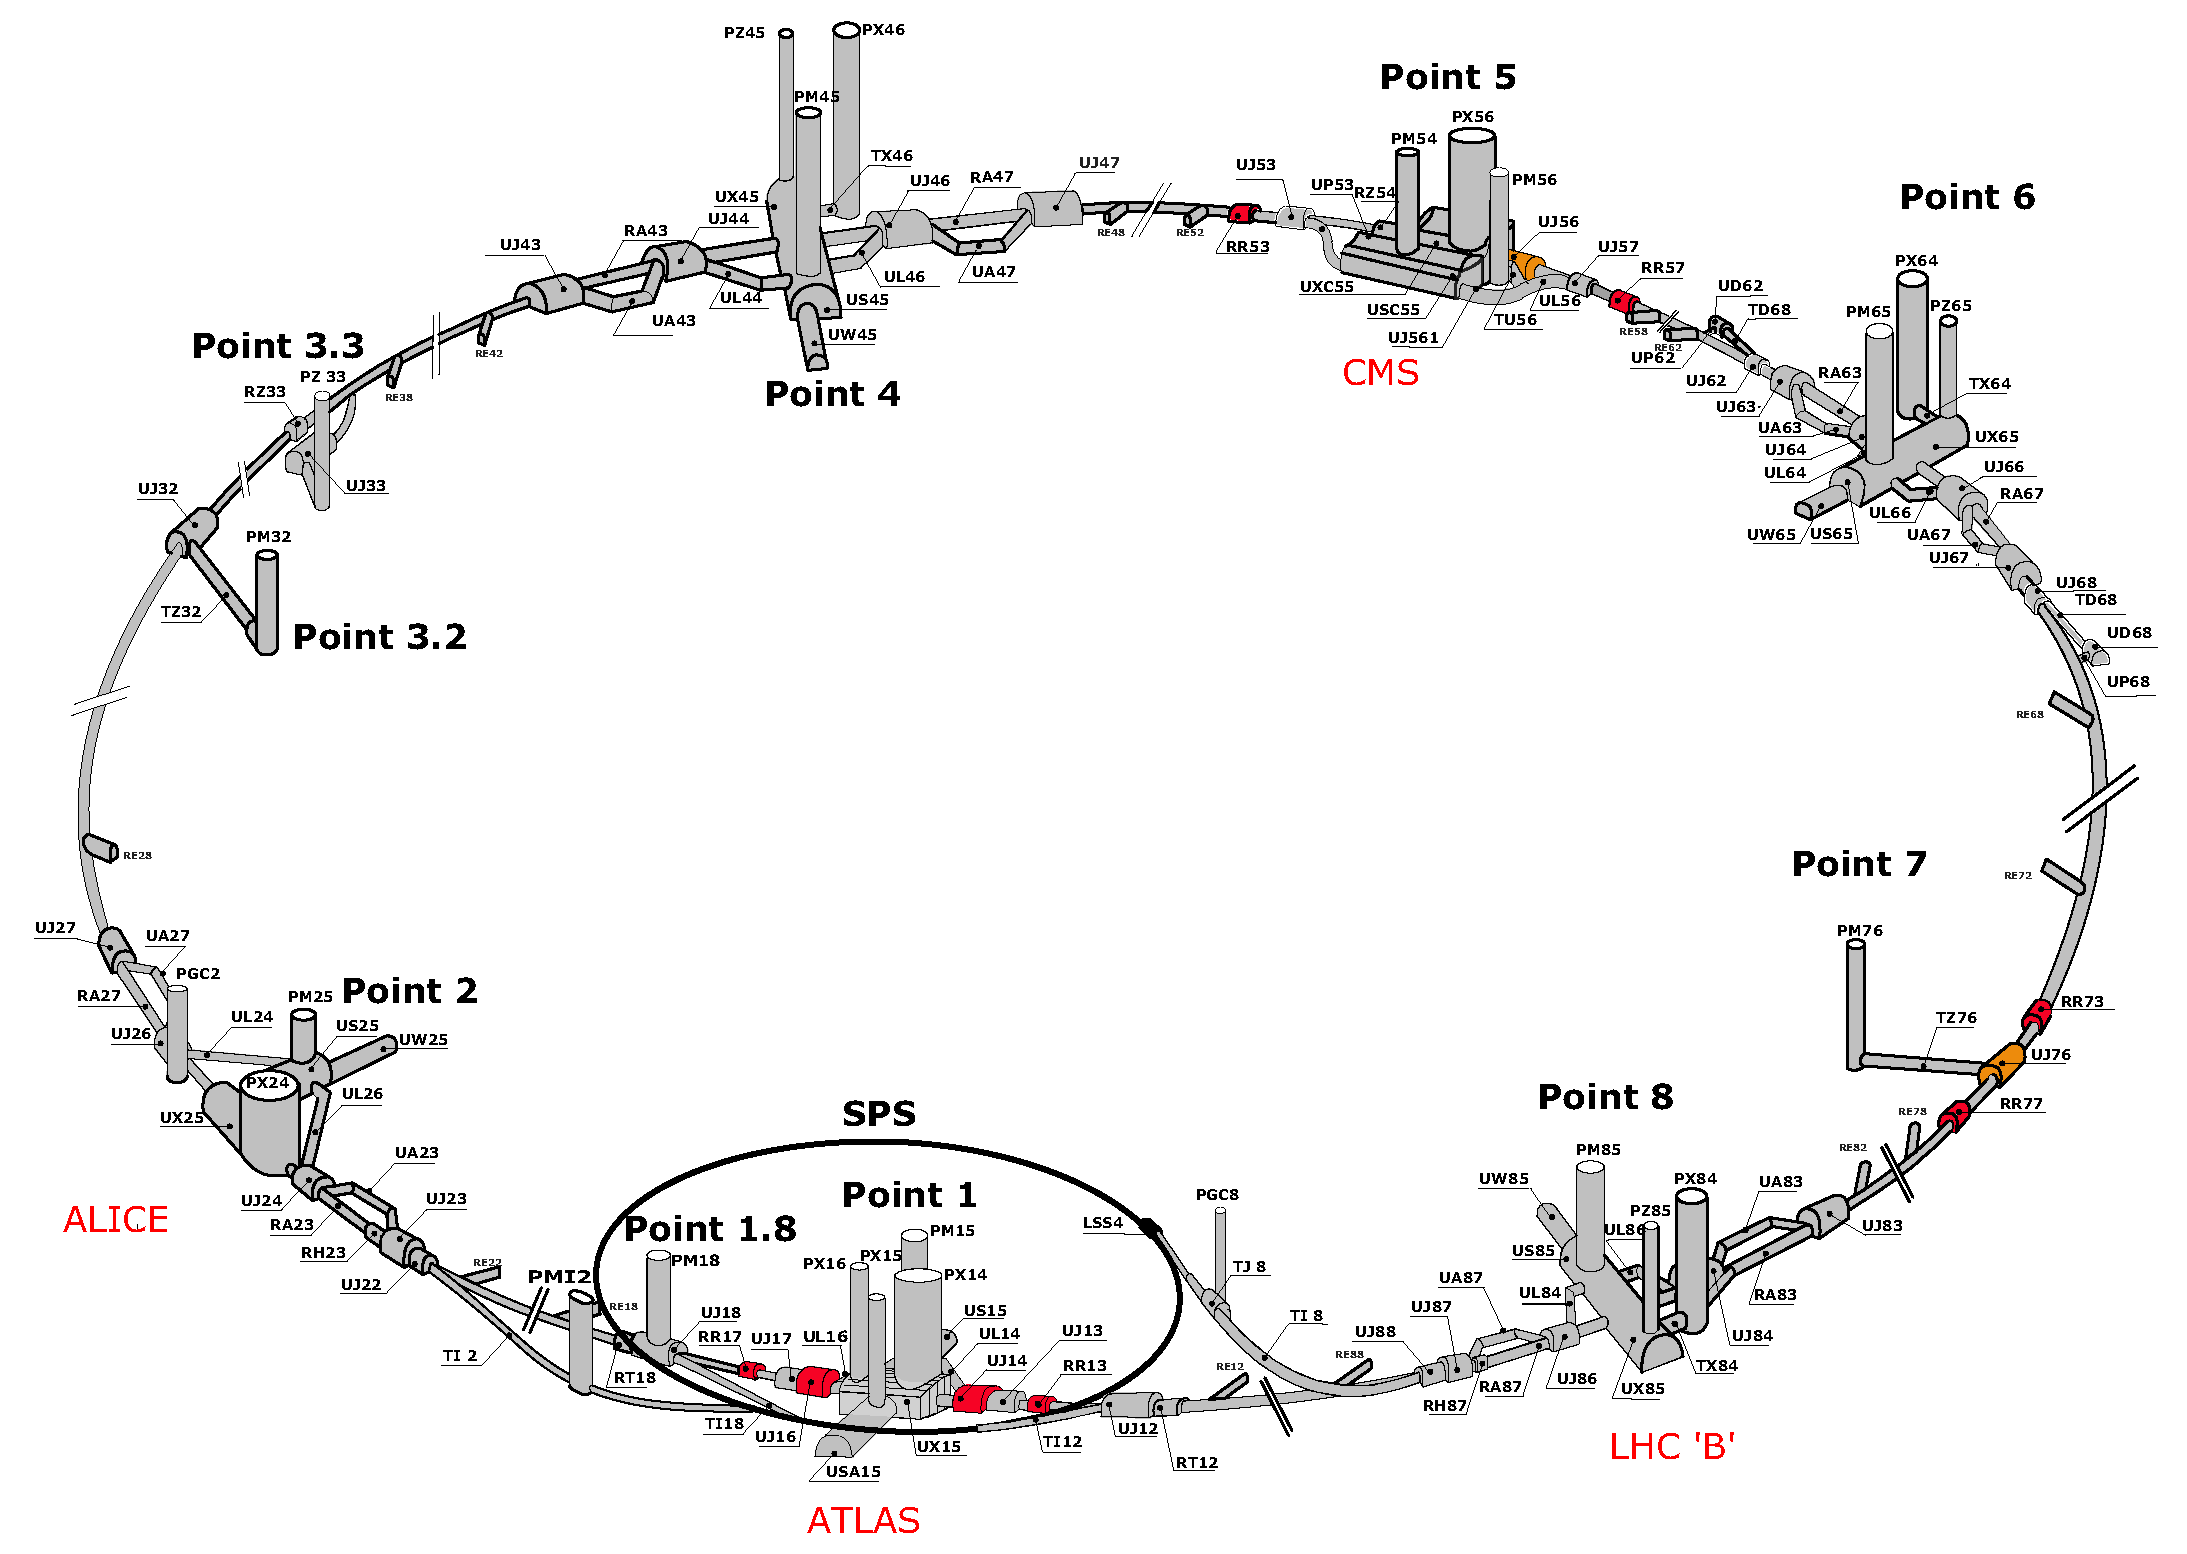
\includegraphics[width=.6\textwidth]{Pictures/LHClayout.PNG}
    \caption{LHC layout [\ref{LHCref}]}
    \label{fig:LHClayout}
\end{figure}

Superconducting magnets in the LHC in the main dipoles of the create a magnetic field of $\approx 8$T to bend the proton beams into the circlular path of the collider. Figure \ref{fig:dipolemagnet} shows the flux in a dipole cross-section. The oposing direction beamlines are shown centered and the flux is shown to be high (and directionally opposed) in center of each beam. To maintain these fields, the magnets operate at below 1.9K. Pressurized superfluid helium, chosen for its low visosity and high specific heat, cools the dipole magnets. Once the two LHC rings are filled from the SPS, center-of-mass energy of the beams increase until they reach peak energy after about 28 minutes. Finally, proton bunches separated by 25ns collide simultaneously in each detector.  

\begin{figure}[!h]
        \centering
    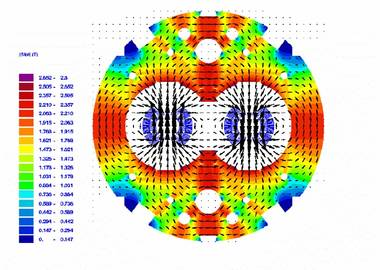
\includegraphics[width=.6\textwidth]{Pictures/dipolemagnet.jpg}
    \caption{ Flux within an LHC dipole cross-section [\ref{LHCref}]}
    \label{fig:dipolemagnet}
\end{figure}

\section{A Toroidal LHC ApparatuS}
\hspace{20pt} The LHC creates proton-proton collisions at a rate and energy level key for pushing the boundaries of particle physics, but identifying and reconstructing the tracks of such energetic particles decay products is no mean feat. A Toroidal LHC ApparatuS (ATLAS) and the Compact Muon Solenoid (CMS) are multi-purpose detectors built to search for and measure a wide range of particle interactions and properties. Both experiments measured a particle consistentwith the Higgs boson in 2012 and their agreement was a key verification of the discovery. The following sections describe each major component of the ATLAS detector with a focus on their use in the measurement of Higgs$\rightarrow WW \rightarrow e\nu\mu\nu$. 

ATLAS utilizes a coordinate system with its origin at the center of the detector (the ``interaction point") and has a z-axis along the beam pipe. The x-axis points from the interaction point to the center of the LHC ring, and the y-axis points upward. The experiment uses cylindrical coordinates $(r, \phi)$ where $\phi$ is the azimuthal angle around the beam pipe. The pseudorapidity and the transverse momentum are defined in terms of the polar angle $\theta$ as $\eta = -\ln( \tan(\theta/2))$ and $p_T = p\sin\theta$. 
\begin{figure}[!h]
	\centering     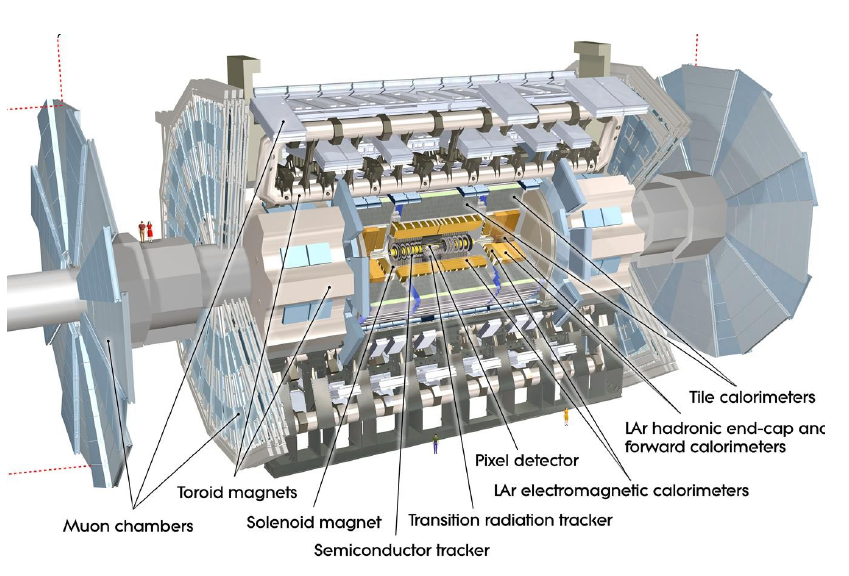
\includegraphics[width=.7\textwidth]{Pictures/ATLASdetector.PNG}
    \caption{Computer-simulated ATLAS detector schematic [\ref{detector}]}
\end{figure}

\par \hspace{20pt} The Inner Detector (ID) detects charged particles with an $|\eta| < 2.5$ operating in a 2T solenoidal field. It consists of $3$ layers of pixel sensors, $4$ layers of silicon strips, and $72$ straw layers of transition radiation tracker modules. The ID describes particles closest to the interaction point and detects track parameters with great resolution due to high granularity. 

The solenoidal magnet... The toroid magnets....

The Muon Spectrometer precision chambers provide muon momentum measurements at a high resolution over a wide range of $p_T$. The MS consists of $3$ layers of Monitored Drift Tube chambers covering $|\eta| < 2.7$ and an inner layer of Cathode Strip Chambers with $|\eta| > 2.0$. In addition, it includes trigger chambers that contain $3$ layers of Resistive Plate Chambers ($|\eta| < 1.05$) and $3$ layers of Thin Gap Chambers ($1.05 < |\eta| < 2.4$). As the outermost subdetector, the MS provides precise muon momentum measurements along the muon trajectory and the muon chambers are located with a precision of under $60$ $\mu m$. The MS also contains a system of three superconducting toroidal magnets each with eight coils providing a magnetic field with a bending integral of up to $6$ Tm. 

Calorimeters provide detailed information about the energy deposited as particles pass through. Electromagnetic calorimeters detect and halt the motion of electrons and photons while the hadronic calorimeter does the same for hadrons. Muons and neutrinos are able to pass through the calorimeters to the MS. The electromagnetic and hadronic calorimeter, made of liquid Argon and scintillating tiles, respectively, are able to pass information from the location of energy deposits to the muon reconstruction algorithm [\ref{detector}]. 

\section{The High-Luminosity LHC and Inner Tracker (ITk)}
Though the LHC succeeded in one of its crucial goals of discovering the Higgs boson in 2012, its continuous operation at higher energy and luminosity has led to more rigorous measurements of the Higgs as well as searches for new physics beyond the Standard Model. The LHC has been the leading high energy collider in terms of person power, energy, and scale for over a decade and will continue to be extremely important for understanding theoretical questions in the future. While more data collection is planned in Run-3 starting in 2021 \textcolor{red}{??}, new colliders and detectors take decades to design, develope and build, so the plans for the collider to take it's place is well underway. The High Luminosity LHC will operate at an LHC-level energy (14TeV) and begin data-taking in 2026. The HL-LHC will begin with $5-7\times$ the luminosity of the LHC and will have a design luminosity of $10\times$ the LHC, or $12.6\times10^{-34}cm^{-2}s^{-1}$. This huge increase in number of collisions requires massive upgrades to the LHC including new, 11-12T superconducting magnet systems, compact superconducting caivities for beam rotation and phase control, and new technology beam collimation \ref{HL-LHC Yellow Paper}. This massive undertaking has been underway for many years already and has involved laboratories all over the world.

Just as the LHC had to be re-designed and built to create higher luminosity, so too do all the experiments on the LHC have to be redesigned to be able to interpret so many more collisions per second. The detectors must be built to withstand more radiation, as the increased collision rate also means a high radiation rate especially closest to the beamline. They also have to provide greater granularity to be able to reconstruct tracks with good enough resolution that individual tracks can be discriminated. Finally, they have to be able to deal with increased pile-up. Pile-up is .. Finally, the increased data in and of itself creates a complex problem for the detectors to solve, as briefly discussed previously, the trigger system must quickly choose which collision events may hold interesting events and store these. When there are more events happening near simultaneously these systems must make these decisions in real-time. New algorithms to speed up this process are necessary when there are an order of magnitude more events to sort through.

Detectors for high energy colliders are not built often- expensive and time-consuming to design and test, they're made to last at least a decade. I was lucky to have the opportunity to work on ATLAS detector research and development during a year I worked at Brookhaven National Laboratory during my Ph.D. and though my thesis isn't directly related to this work, it was formative and extremely interesting, so I'll touch on this work in the next section. Because I worked on the new ATLAS inner detector for the HL-LHC (termed Inner Tracker or ITk) I will just discuss this sub-detector and the particular role I played in its assembly.

\subsection{Inner Tracker (ITk)}
\subsubsection{Building ITk Strip barrel staves}
%This explains why the HL LHC and ITk are necessary+ important, more specifics on my work can be hinted here but go in the
%\subsubsection{ITk strip barrel specifications}
%\subsubsection{Building ITk Strip barrel staves}
%\subsubsection{Thermally testing ITk Strip barrel staves}

